\documentclass{amsdtx}
\usepackage{graphicx}
\usepackage{amsmath}
\usepackage{amssymb}
\usepackage{float}
\usepackage[margin=0.75in]{geometry}
\providecommand{\tightlist}{%
  \setlength{\itemsep}{0pt}\setlength{\parskip}{0pt}}
  \title{\sc Active Control: MIT Rocket Team}
  \author{\small \textbf{\textit{Marc D. NICHITIU, Conrad M. CASEBOLT}}}
  \date{}
\begin{document}
\maketitle

\begin{center}
\textit{Active Control Algorithms and Simulation Testing for MIT Rocket
Team.}
\end{center}

This repository contains tools and code for advanced simulation and
control of rocket flight using both Java (OpenRocket) and Python. The
workflow integrates custom Java simulation logic with Python scripting
and visualization.

\section{Overview}\label{overview}

A Python-based tool for rocket flight simulation that integrates with
OpenRocket to analyze and visualize flight characteristics. This project
focuses on processing and visualizing rocket flight data, particularly
useful for analyzing pitch rates and velocities during flight.

\section{Prerequisites}\label{prerequisites}

\begin{itemize}
\tightlist
\item
  Python 3.12+
\item
  Java Development Kit (JDK) 17
\item
  \texttt{matplotlib}
\item
  \texttt{numpy}
\item
  \texttt{jpype}
\end{itemize}

\section{Environment Setup}\label{environment-setup}

Python Dependencies:
\texttt{pip\ install\ numpy\ matplotlib\ jpype1}

Contact: \verb|nichitiu@mit.edu|

\section{Usage Instructions}

\subsection{Compiling and Running}\label{compiling-and-running}

\begin{itemize}
\tightlist
\item
  \textbf{Use the \texttt{OR\_interfaceTest\ +\ JAR} run configuration}
  in your IDE to:

  \begin{itemize}
  \tightlist
  \item
    Compile the Java code (including your modifications).
  \item
    Run the Python script that interfaces with the compiled Java
    classes.
  \end{itemize}
\end{itemize}

\subsection{Editing Simulation and Control
Logic}\label{editing-simulation-and-control-logic}

\begin{itemize}
\item
  \textbf{Simulation Flow:}\\
  Edit only \texttt{ModifiedEventSimulationEngine.java} to manage the
  overall simulation flow, such as event handling, simulation stepping,
  and integration with listeners.
\item
  \textbf{Controller Behavior:}\\
  Edit \texttt{NewControlStepListener.java} to modify the controller's
  behavior and properties. This file is responsible for how the control
  system interacts with the simulation at each step.
\item
  \textbf{Python Scripting:}\\
  Edit \texttt{openRocketInterface.py} (located in \texttt{sim/src/py/}
  or similar) to change how the Python script interacts with the Java
  code. This script is used to run specific tests, automate simulation
  runs, and collect results.
\end{itemize}

\section{\texorpdfstring{Python Script:
\texttt{openRocketInterface.py}}{Python Script: openRocketInterface.py}}\label{python-script-openrocketinterface.py}

This script uses \texttt{jpype} to launch the JVM and interface directly
with the compiled Java classes. It allows you to:

\begin{itemize}
\item
  \textbf{Control Java Variables:}\\
  The script can set and get various simulation parameters in Java, such
  as:

  \begin{itemize}
  \tightlist
  \item
    Time step size (variable \texttt{prefDt} in
    \texttt{openRocketInterface.py})
  \item
    Controller gains and setpoints
  \item
    Initial conditions (e.g., launch angle, velocity)
  \item
    Simulation duration and event triggers
  \end{itemize}
\item
  \textbf{Run and Automate Simulations:}\\
  You can script multiple runs, parameter sweeps, or custom test
  scenarios by calling Java methods from Python.
\item
  \textbf{Graphing and Visualization:}\\
  The script collects simulation output (e.g., altitude, velocity,
  control surface deflections, error signals) and generates plots for
  analysis. The default graph plots two panels, showing

  \begin{itemize}
  \tightlist
  \item
    Altitude, Velocity vs.~time
  \item
    Control output (fin cant) and rotational velocity vs.~time
  \end{itemize}
\end{itemize}

\section{Repository File Structure}\label{repository-file-structure}

This repository is organized as follows:

\begin{itemize}
\item
  \texttt{README.md} Project documentation and usage instructions.
\item
  \texttt{bib/}\strut \\
  Reference materials and research papers.
\item
  \texttt{canard/}, \texttt{ctrl/}, \texttt{wing/}\\
  Subdirectories for specific rocket components, control models, and
  aerodynamic studies.
\item
  \texttt{clone/}\strut \\
  Contains OpenRocket source code and related files:

  \begin{itemize}
  \tightlist
  \item
    \texttt{openrocket/} and \texttt{openrocket-release-24.12.RC.01/}\\
    OpenRocket Java source, build scripts, and documentation.
    \texttt{openrocket/} is a symlink to the openrocket version used,
    currently \texttt{openrocket-release-24.12.RC.01/}.
  \end{itemize}
\item
  \texttt{land.tbd/}\strut \\
  Landing simulation (tbd - i.e.~in progress) documentation and related
  files.
\item
  \texttt{sim/}\strut \\
  Main simulation code and data:

  \begin{itemize}
  \tightlist
  \item
    \texttt{src/py/}\strut \\
    Python scripts for simulation and Java-Python integration (e.g.,
    \texttt{openRocketInterface.py}).
  \end{itemize}
\item
  \texttt{src/java/}\strut \\
  A symlink to the Java source of the used openrocket distribution - for
  ease of navigation.
\item
  \texttt{dat/}\strut \\
  Simulation results and data output.
\item
  \texttt{stabil/}\strut \\
  Additional files pertaining to the roll controller, mostly ideation.
\item
  \texttt{test/}\strut \\
  Test scripts and utilities.
\end{itemize}

Each directory contains files relevant to its purpose, such as source
code, data, documentation, or research materials. The main simulation
workflow is in the \texttt{sim/} directory, with integration to Java
code in \texttt{clone/openrocket-release-24.12.RC.01/}.
\newpage
\section{Sample Output}
\subsection{Setup}
Below is a comparison of the \verb|RK4| and \verb|RK6| integration methods for controller stability. The control coefficients used are:
\begin{multicols}{4}
\begin{itemize}
  \item $k_P=2.0$
  \item $k_I=0.75$
  \item $k_D=0.226$
  \item $v_{\rm min}=15$ m/s
\end{itemize}
\end{multicols}
The controller will thus use a PID controller (see below) when the rocket's vertical velocity is larger than 15 m/s. We also note that the controller is only applied on ascent. Here, the controller's ``ideal'' rotational velocity is \textbf{zero}. Let $f(t)$ be the fin cant at some time $t$. Let the simulation step be $dt$. Let $\omega_0$ be the desired rotational velocity (here $0$), and let $\omega(t)$ be the measured rotational velocity. Thus, the controller uses the following equation to calculate the next fin cant:
\begin{align}
  f(t+dt) = (\omega_0-\omega(t))k_P + (\omega(t-dt)-\omega(t))k_D + k_I\sum_j(\omega_0-\omega(t-jdt))
\end{align}
Note that fin cant is capped at 15$^\circ$ in the \verb|openrocket| framework.

As a sample rocket, we use that described by the file `sim/dat/ork/demonstrator_1.ork`.
\subsection{Results}
Upon simulation with varying timesteps, it is possible to observe an ameliorated modeling of the controller. In the graphs below, at left is an \verb|RK4| simulation, and at right is an \verb|RK6| simulation. Note that in each graph, the angular velocity scale (bottom panel, left side) uses a \verb|linlog| scale that is logarithmic for values larger than $10^{-3}$ in absolute value and linear for values less than $10^{-3}$ in absolute value. Also note that the horizontal black dotted line in the upper panel denotes the minimum velocity threshold for controller engagement, noted above to be $15$ m/s.
\begin{figure}[H]
\centering
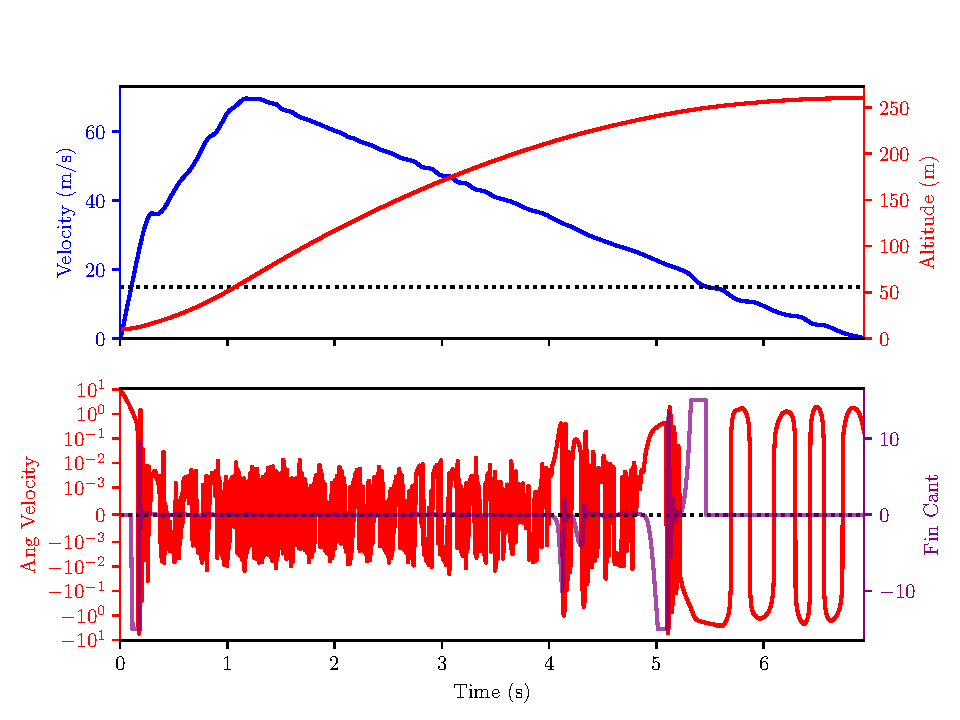
\includegraphics[width=0.4\textwidth]{bib/figures_for_readme/RK4_dt_0p001.pdf}
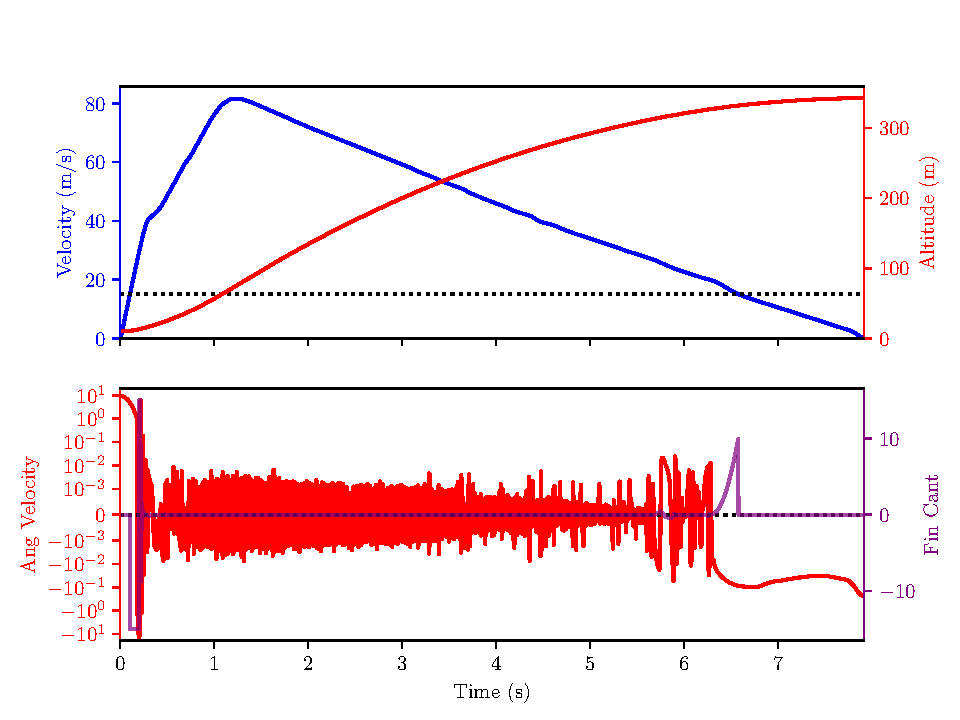
\includegraphics[width=0.4\textwidth]{bib/figures_for_readme/RK6_dt_0p001.pdf}
\caption{$dt=10^{-3}$}
\end{figure}
\begin{figure}[H]
\centering
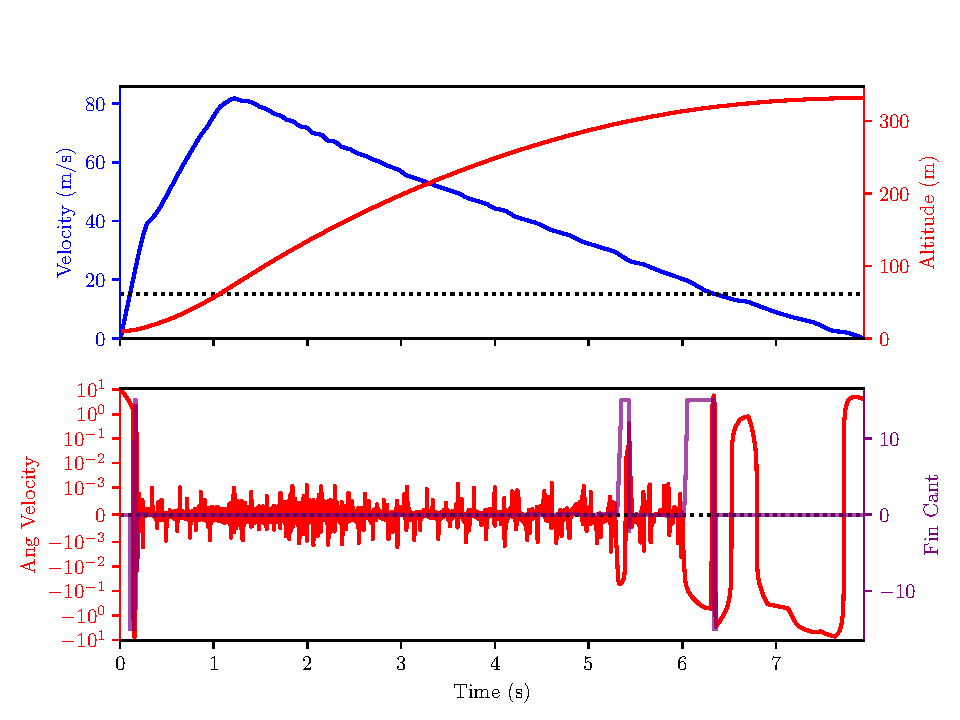
\includegraphics[width=0.4\textwidth]{bib/figures_for_readme/RK4_dt_0p0001.pdf}
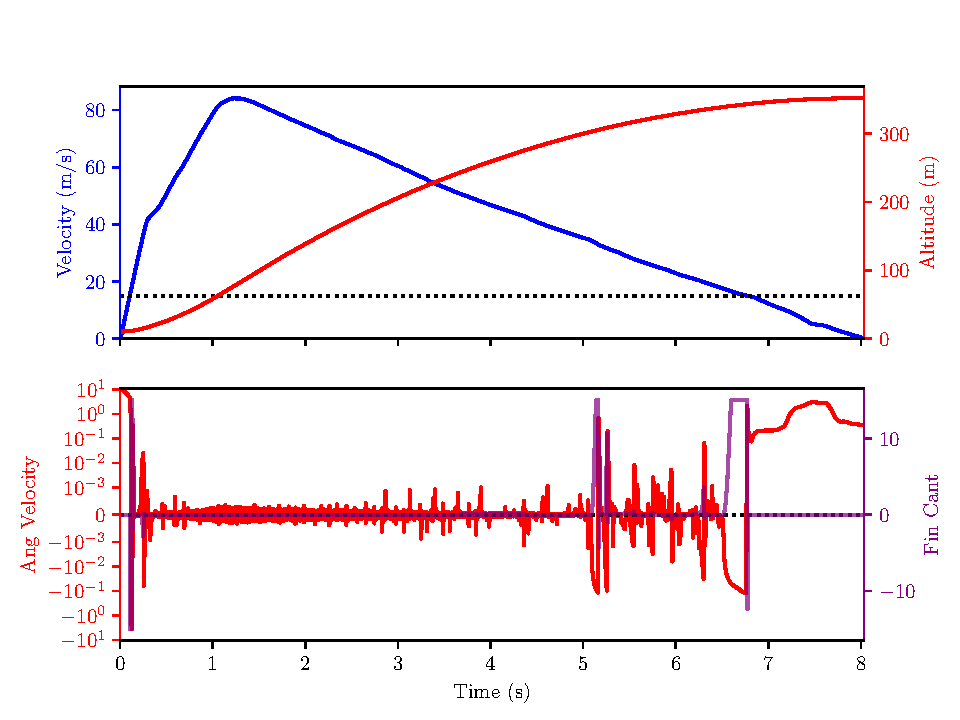
\includegraphics[width=0.4\textwidth]{bib/figures_for_readme/RK6_dt_0p0001.pdf}
\caption{$dt=10^{-4}$}
\end{figure}
\begin{figure}[H]
\centering
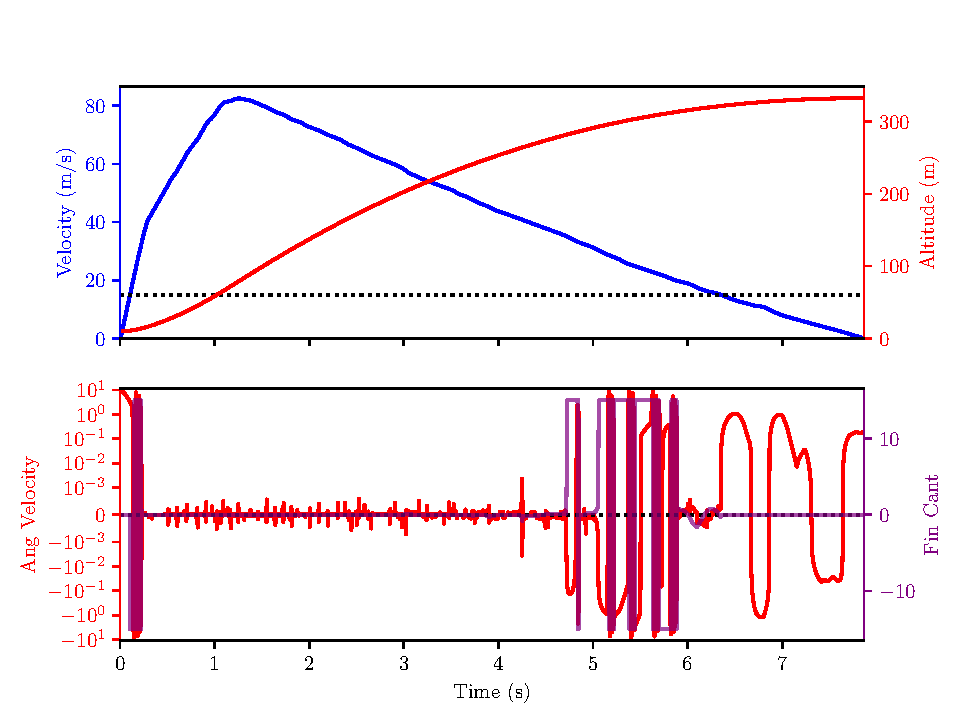
\includegraphics[width=0.4\textwidth]{bib/figures_for_readme/RK4_dt_0p00001.pdf}
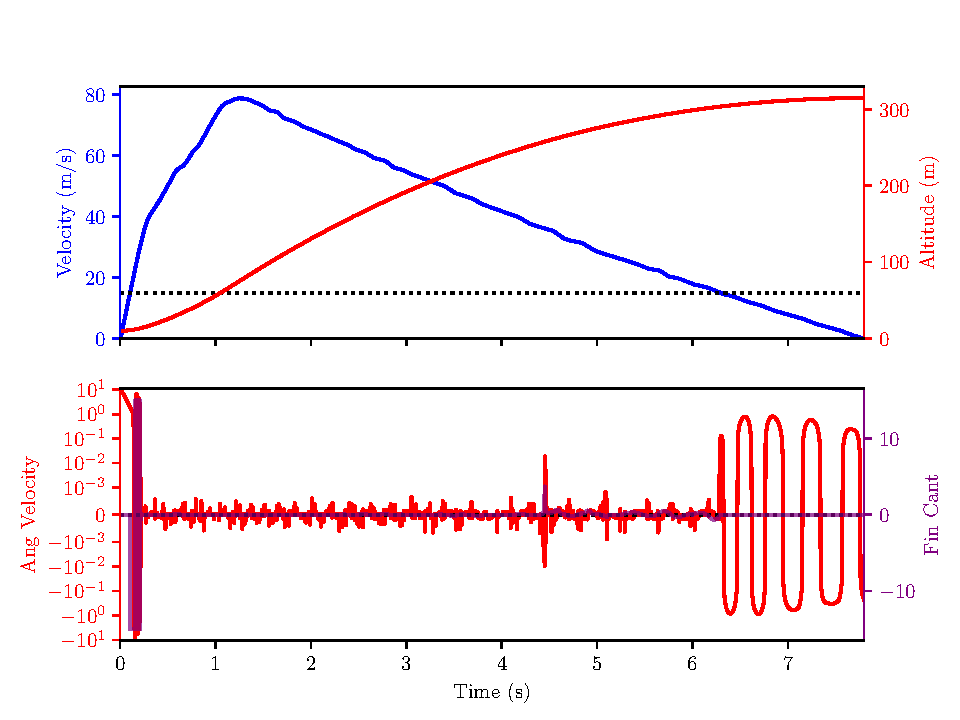
\includegraphics[width=0.4\textwidth]{bib/figures_for_readme/RK6_dt_0p00001.pdf}
\caption{$dt=10^{-5}$}
\end{figure}







\end{document}







